\documentclass{article}
\usepackage[utf8]{inputenc}
\usepackage[dvipdfmx]{hyperref}
\usepackage{fancyhdr}
\usepackage{caption, floatrow}

\usepackage[dvipdfmx]{graphicx}

\usepackage{mathtools}
\renewcommand{\theequation}{eq. \arabic{equation}}


\usepackage[
  style=numeric,
  citestyle=numeric,
  url=true,
  doi=false,
  isbn=false
  ]{biblatex}
\addbibresource{main.bib}


\DeclareNewFloatType{graph}{placement=H, name=Graph}
\floatsetup[graph]{capposition=bottom}


% contents below
% ------------------------------------------------------------------------------

\pagestyle{fancy}
\fancyhf{}
\rhead{Rikuo Hasegawa}
\chead{UPCSE PHYSICS Short Lab Report}
\lhead{\today}
\rfoot{p. \thepage}

\title{Measurement of charge to mass ratio of an electron using mass spectrometry}
\author{ Rikuo Hasegawa
  \\ Tutorial Group: C
  \\ Lab Group: C2 }

\begin{document}

\maketitle
\thispagestyle{fancy}
\vspace*{\fill}
\parbox{\linewidth}{\centering%
Date of Experiment: May 1st, 2019
}
\newpage


\section{Introduction}
\paragraph{}
In this experiment our goal was to measure the charge to mass ratio of an electron by taking measurements using mass spectrometry.

\section{Theory}
\paragraph{}
An electron with charge \(e\) traveling through a uniform electric field \(\vec{E}\) is subject to a force \(\vec{F_E}\) given in \eqref{electric_force}.

\begin{equation}\label{electric_force}
  \vec{F_E} = -e\vec{E}
\end{equation}

The same electron (w.r.t charge) travelling through a uniform magnetic field \(\vec{B}\) at velocity \(\vec{v}\) is subject to a force \(\vec{F_B}\) given in \eqref{magnetic_force}.

\begin{equation}\label{magnetic_force}
  \vec{F_B} = e(\vec{v}\times\vec{B})
\end{equation}

These are visualized in Figure \ref{fig:forces}.

\begin{figure}[h]
  \includegraphics{./img/Capture.pdf}
  \caption{Visualization of electric and magnetic fields}
  \label{fig:forces}
\end{figure}

If the magnetic field and electric field are perpendicular to the velocity of the electron and each other, the two forces can be along the same axis and therefore cancel out when the conditions in \eqref{cancel}  are met.

\begin{equation}\label{cancel}
  e|\vec{E}| = e|\vec{v}||\vec{B}|
\end{equation}

In this experiment the electrons are accelerated using an electron gun through an electric potential difference \(V_a\). The kinetic energy of the electron can then be determined from the voltage of this potential difference as shown in \eqref{kinetic}

\begin{equation}\label{kinetic}
  \frac{1}{2} m v^2 = eV_a
\end{equation}

Shuffling the variables around yields \eqref{simple_ratio}

\begin{equation}\label{simple_ratio}
  \frac{e}{m} = \frac{v^2}{2V_a}
\end{equation}

\section{Experimental Equipment and Method}
\subsection{Apparatus}
\paragraph{}

The apparatus is shown in Figure \ref{fig:picture} and illustrated in Figure \ref{fig:apparatus}. The main components are listed below:

\begin{itemize}
  \item Electron gun
  \item Helmholtz coils placed 6.9 cm apart from each other.
  \item Electric plates (inside the glass sphere where the electrons travel)
  \begin{itemize}
    \item separated by 8.0mm
  \end{itemize}
  \item Power supplies for each of the above
  \item Digital Voltmeters for \(V_a\) and \(V_p\) (explained below)
  \item Luminescent screen inside the glass sphere
\end{itemize}

\begin{figure}[H]
  \includegraphics[width=\textwidth]{./img/pictor.pdf}
  \caption{The experiment apparatus \autocite{UPCSE2018}}
  \label{fig:picture}
\end{figure}

\begin{figure}[H]
  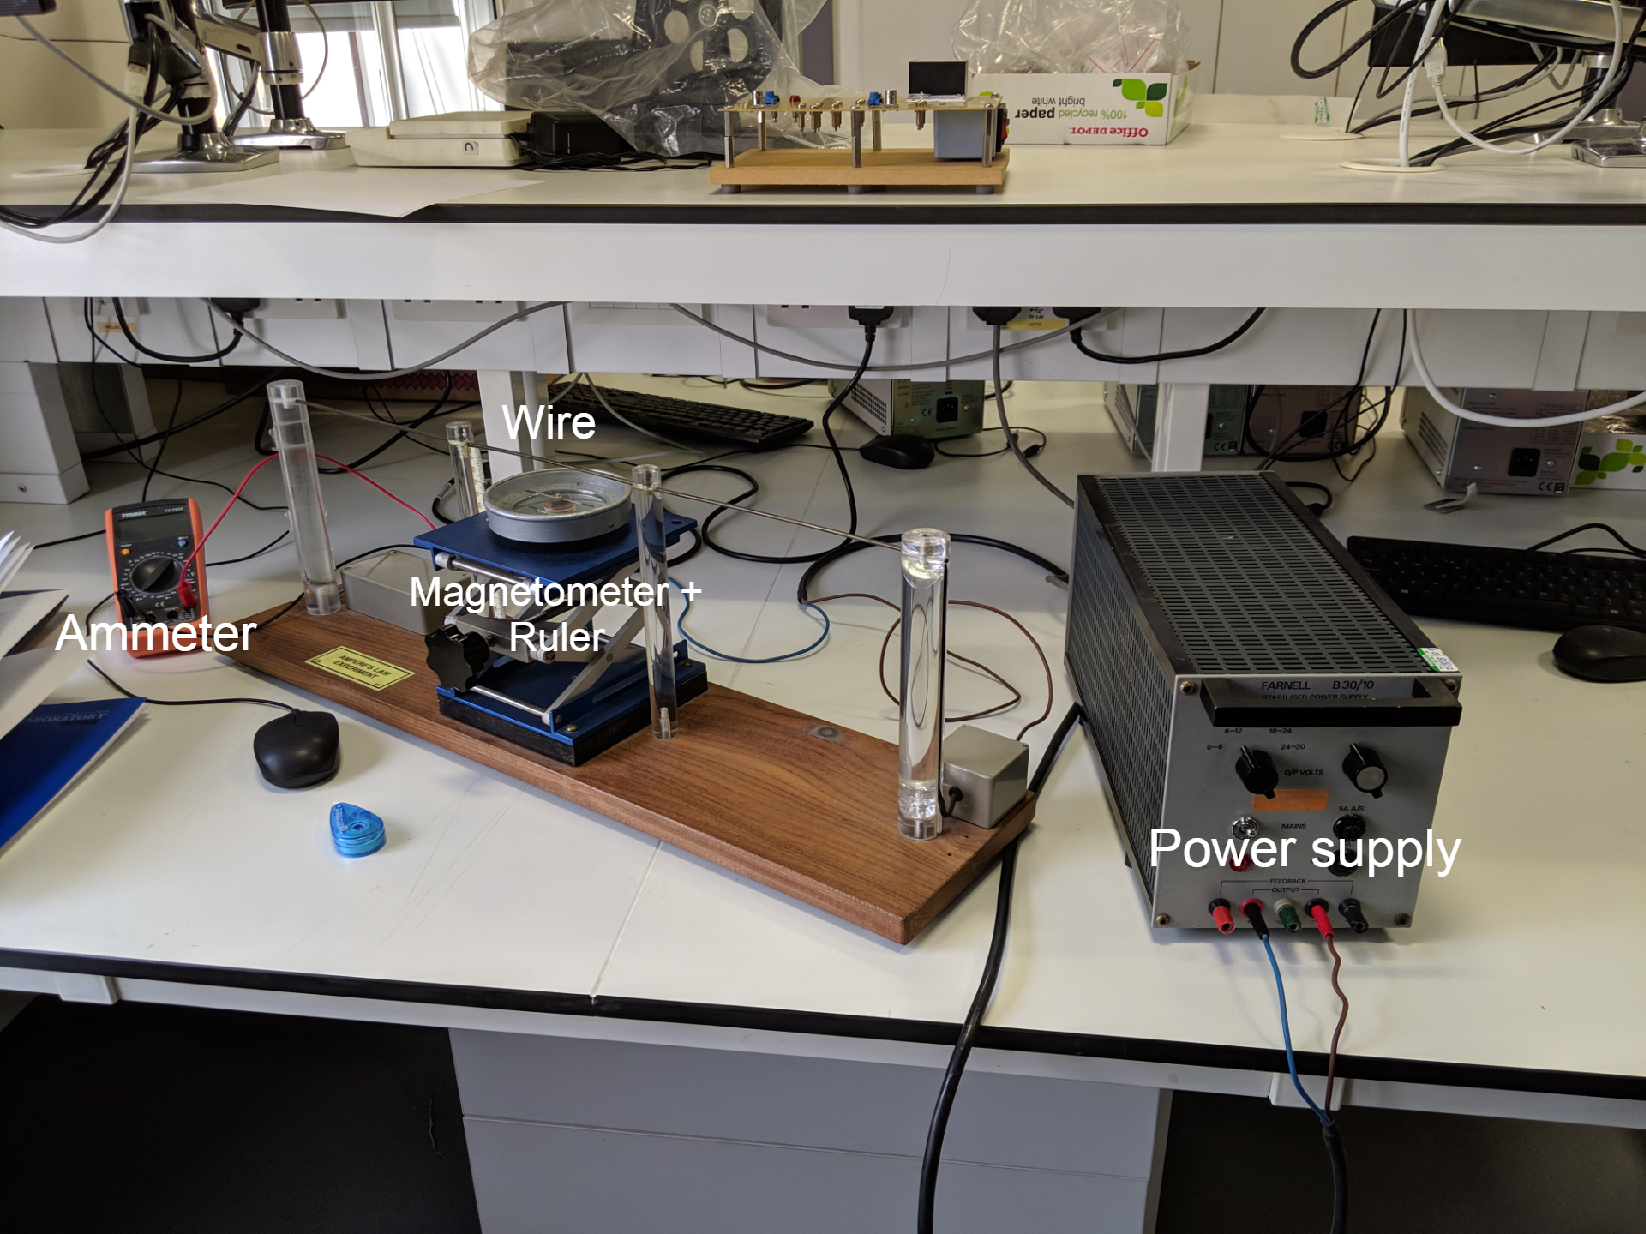
\includegraphics[width=\textwidth]{./img/apparatus.pdf}
  \caption{A diagram of the apparatus \autocite{UPCSE2018}}
  \label{fig:apparatus}
\end{figure}

The magnetic field from the pair of Helmholtz coils \(B\) is derived by \eqref{magnetic_field}.
\begin{equation}\label{magnetic_field}
  B=kI_h
\end{equation}
where \(k = 4.17\times10^{-3} ~TA^{-1}\) and \(I_h\) is the current flowing through the coils.

The electric field \(E\) between the plates is given by \eqref{electric_field}.
\begin{equation}\label{electric_field}
  E=\frac{V_p}{d}
\end{equation}
where \(V_p\) is the potential difference between the plates and \(d\) is the distance between the plates (in this experiment, the plates are 8.0 mm apart from each other.).

\subsection{Protocol}
\paragraph{}
The experimental protocol is described below:

\begin{enumerate}
  \item Configure all the equipment according to the schematic in Figure \ref{fig:schematic}
  \item Set the voltage of the electron gun \(V_a\) to 3000V
  \begin{itemize}
    \item Note that the Monitor voltage is always DC regardless of the actual voltage.
  \end{itemize}
  \item Main Measurement loop (parameters: \(V_a \in [50, 300]\) and \(I_h\) [dependent variable])
  \begin{enumerate}
    \item Set \(V_a\)
    \item Adjust \(I_h\) so the beam is straight and hits the opposite corner of the luminescent screen.
    \item Take a measurement of that current.
  \end{enumerate}
\end{enumerate}

\begin{figure}[h]
  \includegraphics[width=\textwidth]{./img/schematic.pdf}
  \caption{Schematic diagram of wiring for apparatus \autocite{UPCSE2018}}
  \label{fig:schematic}
\end{figure}

\section{Results}
\paragraph{}
Our raw measurements are shown in Table \ref{tb:results}.

\begin{table}[H]
  \caption{Raw measurements of \(I_h\) and \(V_a\)}
  \label{tb:results}
  \begin{tabular}{|c|c|}
  \hline
  \multicolumn{1}{|l|}{\textbf{Vp {[}V{]}}} & \multicolumn{1}{l|}{\textbf{Ih {[}A{]}}} \\ \hline
  \(5.00 \times 10^1\)                                  & \(4.90 \times 10^{-2}\)                                 \\ \hline
  \(7.50 \times 10^1\)                                  & \(7.30 \times 10^{-2}\)                                 \\ \hline
  \(1.00 \times 10^2\)                                  & \(9.70 \times 10^{-2}\)                                 \\ \hline
  \(1.25 \times 10^2\)                                  & \(1.30 \times 10^{-1}\)                                 \\ \hline
  \(1.50 \times 10^2\)                                  & \(1.54 \times 10^{-1}\)                                 \\ \hline
  \(1.75 \times 10^2\)                                  & \(1.90 \times 10^{-1}\)                                 \\ \hline
  \(2.00 \times 10^2\)                                  & \(2.10 \times 10^{-1}\)                                 \\ \hline
  \(2.25 \times 10^2\)                                  & \(2.37 \times 10^{-1}\)                                 \\ \hline
  \(2.50 \times 10^2\)                                  & \(2.64 \times 10^{-1}\)                                 \\ \hline
  \(2.75 \times 10^2\)                                  & \(2.92 \times 10^{-1}\)                                 \\ \hline
  \(3.00 \times 10^2\)                                  & \(3.14 \times 10^{-1}\)                                 \\ \hline
  \end{tabular}
\end{table}

The graph of \(I_h\) plotted against \(V_p\) is shown in Graph \ref{g:graph}

\begin{graph}[H]
  \includegraphics[width=\textwidth]{./img/graph.pdf}
  \caption{Current in coil against plate voltage}
  \label{g:graph}
\end{graph}

By combining \eqref{simple_ratio} with \eqref{magnetic_field} and \eqref{electric_field} we get \eqref{final}

\begin{equation}\label{final}
  \frac{e}{m} = \cfrac{V_p^2}{2d^2k^2I_h^2V_a}
\end{equation}

From \eqref{final} we can get \eqref{grad}

\begin{equation}\label{grad}
  G = \sqrt{\frac{m}{e} \times 4.49 \times 10^8 \times \frac{1}{V_a}}
\end{equation}

Which describes the gradient \(G\) of the graph.

\section{Uncertainty Analysis}
\paragraph{}
By using the Data Analysis package in Microsoft Excel, we measured the following values for the lower and upper 95\% confidence for the gradient of Graph \ref{g:graph}.

\[
  G \in [0.00105, 0.00111]
\]

Therefore, the random error on our gradient will be:

\[
  \Delta G = 3 \times 10^{-5}
\]

Using these values, our final measurement of the charge to mass ratio is given below:

\[
  \frac{e}{m} = 1.28 \times 10^{11} \pm 6.5 \times 10^{9} ~\text{[C/Kg]}
\]

\section{Discussion and Conclusion}
\paragraph{}

Our results seem to somewhat agree with the known measurements for the electron charge to mass ratio of \( 1.75 \times 10^{11} ~\text{[C/Kg]}\) \autocite{mohr2016} (not an order of magnitude off). But our measurements seem to have some systematic errors.

Some possible reasons for this error could be due to the fact that we could not configure our Helmholtz coils precisely parallell at a distance of 6.9 cm apart. This could potentially affect the constant \(k\) since the value was most likely measured experimentally for the conditions described in the lab book.

Another potential source of error is from the thickness of the beam since the beam was very sensitive to perturbances in the coil current, the variance in the value for \(I_h\) is quite high from one edge of the beam to the other. We tried our best to align the center of the beam to the corner of the screen but that may have been a cause of error, although that should probably lead to a random error unless the operator was biased to offset the beam in a particular direction.

In conclusion, the experiment was a failure as it failed to capture the true value of the electron charge to mass ratio but we have identified some potential problems for future experiments.

\printbibliography
\end{document}
